\documentclass[conference]{IEEEtran}
\IEEEoverridecommandlockouts
\usepackage{cite}
\usepackage{amsmath,amssymb}
\usepackage{graphicx}
\usepackage{booktabs}
\usepackage{multirow}
\usepackage{array}
\usepackage{algorithm}
\usepackage{algpseudocode}
\usepackage{xcolor}
\usepackage{tikz}
\usetikzlibrary{arrows.meta,positioning,fit,calc}
\usepackage{url}
\IfFileExists{xurl.sty}{\usepackage{xurl}}{}
\usepackage[hidelinks]{hyperref}

\newcommand{\NEI}{\textsc{nei}}
\newcommand{\NA}{\textsc{n/a}}
\algrenewcommand\algorithmicrequire{\textbf{Input:}}
\algrenewcommand\algorithmicensure{\textbf{Output:}}

\begin{document}

\title{TrialMatch: Evidence-Grounded Criterion-Level Clinical Trial Screening with a LoRA-Adapted Small Language Model and Hand-Implemented Efficient Decoding}

\author{\IEEEauthorblockN{Eshaal Malik}
\IEEEauthorblockA{Roll No.\ 23I-0732\\
FAST School of Computing, National University of Computer and Emerging Sciences (FAST-NUCES)\\
Islamabad, Pakistan}}

\maketitle

\begin{abstract}
Clinical trial screening requires deciding, criterion by criterion, whether a patient record satisfies a trial's inclusion and exclusion rules, and showing which sentences support each decision. This paper presents TrialMatch, an end-to-end system built on the TrialGPT Criterion Annotations benchmark with the prescribed 37/8/8 patient-grouped split. Qwen2.5-1.5B-Instruct is adapted with Low-Rank Adaptation (LoRA; 18.5\,M trainable parameters) to emit a JSON object containing supporting sentence IDs and one of the six expert label categories. On the 206 held-out test annotations, fine-tuning raises accuracy from 0.267 to 0.733 and macro-F1 from 0.173 to 0.468 (patient-level bootstrap 95\% CI of the gains: $+$0.33 to $+$0.58 and $+$0.21 to $+$0.37), and evidence micro-F1 from 0.136 to 0.601. The model nevertheless beats a majority-label baseline (0.626) mainly on inclusion criteria; it never predicts the rare \emph{not included}, \emph{excluded} and \emph{not applicable} classes, which we analyse as the main limitation. We also implement, from the model's weights upward, a decoder that owns its key/value (KV) cache, a tiled attention kernel with online softmax, and greedy speculative decoding with a 0.5B draft. All three are validated against reference paths: KV-cached and speculative decoding reproduce greedy tokens exactly in FP32, and the residual BF16 differences are traced to one-ulp logit ties. KV caching speeds up decoding by about 32$\times$ at 1{,}024 input tokens, tiled attention cuts attention memory 57$\times$ at 4{,}096 tokens while running slower than a fused kernel, and speculative decoding reaches a 0.94 acceptance rate yet remains slower than greedy decoding (0.77$\times$), which a cost model explains. A browser application exposes screening, evidence inspection, report export and a live decoding benchmark.
\end{abstract}

\begin{IEEEkeywords}
clinical trial matching, eligibility criteria, large language models, LoRA, KV cache, online softmax, tiled attention, speculative decoding, evidence retrieval
\end{IEEEkeywords}

% ======================================================================
\section{Introduction}
Recruitment is one of the main causes of delay in clinical trials, and much of the effort goes into screening: reading a patient's record against dozens of free-text eligibility criteria. Large language models (LLMs) can read both kinds of text, and TrialGPT showed that GPT-4 can predict criterion-level eligibility and cite the supporting patient sentences~\cite{jin2024trialgpt}. Proprietary APIs, however, cannot be inspected, fine-tuned or run locally on patient data, and a screening tool that cannot say \emph{why} it reached a decision is hard to trust.

This work asks whether a small, open-weight decoder that fits a free Colab Tesla T4 GPU can be adapted to the same criterion-level task, and whether the inference machinery behind fast decoding can be implemented and verified rather than switched on through a library flag. Given (i) a patient note split into numbered sentences, (ii) a criterion type and (iii) the criterion text, the model must return one of the expert label categories together with the IDs of the supporting sentences. We keep all expert categories, including \emph{not enough information} (\NEI) and \emph{not applicable} (\NA), so that missing information is never silently turned into a decision.

The contributions are:
\begin{itemize}
\item A LoRA-adapted Qwen2.5-1.5B-Instruct model with a structured, evidence-first output schema, evaluated before and after fine-tuning on the fixed patient-grouped split with classification and evidence metrics, patient-level bootstrap intervals, a majority baseline and an error taxonomy.
\item A from-scratch decoder forward pass (RoPE, grouped-query attention, causal masking with query offset) that owns a pre-allocated KV cache, verified token-for-token against uncached decoding.
\item A tiled attention kernel with online softmax and causal block skipping, validated against an FP64 reference over 16 shape/precision cases.
\item Greedy speculative decoding with explicit cache rollback, verified to match greedy target decoding exactly, together with an analysis of why it is slower on this hardware.
\item A browser application for screening, evidence inspection, report export and live benchmarking, plus a documented account of the difficulties encountered (emulated BF16 on the T4, a hidden repetition penalty in the model's default generation configuration).
\end{itemize}

% ======================================================================
\section{Related Work}
\textit{Clinical trial matching.} Koopman and Zuccon released the SIGIR 2016 test collection of patient topics and trials~\cite{koopman2016}, from which the patients in TrialGPT's criterion annotations are drawn. TrialGPT~\cite{jin2024trialgpt} prompts GPT-4 to judge each criterion, cite evidence sentences and aggregate the results into trial rankings; its expert annotations are the benchmark used here, but its GPT-4 predictions are excluded from all inputs. Wong et~al.\ scaled LLM-based matching to oncology trials and reported that structured, criterion-level prompting helps, but they also relied on proprietary models~\cite{wong2023scaling}. TrialMatch differs by fine-tuning a 1.5B open model that runs locally, and by evaluating evidence localisation with explicit handling of empty evidence sets.

\textit{Small open decoders and parameter-efficient adaptation.} The Transformer~\cite{vaswani2017} underlies all models considered. Qwen2.5~\cite{qwen25}, Llama~3~\cite{llama3} and SmolLM2~\cite{smollm2} offer models between 0.5B and 3B parameters. Rotary position embeddings (RoPE)~\cite{su2024roformer} and grouped-query attention (GQA)~\cite{ainslie2023gqa}, which generalises multi-query attention~\cite{shazeer2019}, determine how positions and the KV cache must be handled during decoding. LoRA~\cite{hu2022lora} trains low-rank updates to frozen weights; QLoRA~\cite{dettmers2023qlora} additionally quantises the frozen base. With a 1.5B model the base fits in 16-bit precision on a T4, so plain LoRA was preferred and quantisation error was avoided.

\textit{Efficient inference.} Pope et~al.\ analyse autoregressive inference as memory-bandwidth bound and motivate KV caching and multi-query attention~\cite{pope2023}; PagedAttention manages cache memory at serving scale~\cite{kwon2023paged}. The online softmax of Milakov and Gimelshein~\cite{milakov2018} computes softmax normalisers in one pass; Rabe and Staats showed that attention can be computed in constant memory per query by chunking~\cite{rabe2021}; FlashAttention~\cite{dao2022flash,dao2023flash2} fuses this tiling into one GPU kernel. Speculative decoding~\cite{leviathan2023,chen2023spec} uses a small draft model to propose tokens that a target model verifies in one pass, preserving the target's output distribution (exactly, in the greedy case). Our implementations follow these papers, but are written in plain PyTorch on top of Hugging Face Transformers~\cite{wolf2020transformers} so that each step can be inspected and tested.

% ======================================================================
\section{Materials and Methods}

\subsection{Dataset, Cleaning and Patient-Grouped Split}
The TrialGPT Criterion Annotations dataset contains 1{,}015 criterion-level annotations for 53 SIGIR patients and 103 trials. Each row holds a numbered patient note, a criterion type (inclusion/exclusion), the criterion text, an expert label and the expert's evidence sentence IDs. Immediately after loading, the four GPT-4 columns (\texttt{gpt4\_explanation}, \texttt{explanation\_correctness}, \texttt{gpt4\_sentences}, \texttt{gpt4\_eligibility}) are dropped, and the dataset's own \texttt{training} flag is ignored. One row with an empty criterion was removed; no label was inconsistent with its criterion type and no evidence ID was out of range, leaving 1{,}014 annotations.

Following the protocol, unique patient IDs were sorted, shuffled with \texttt{numpy.random.default\_rng(42)}, and assigned 37/8/8 to train/validation/test (Table~\ref{tab:split}). Automated checks confirmed that no patient, identical note, or identical (note, criterion) pair occurs in more than one split. The manifest with patient IDs and per-patient counts is published in the repository. The test split contains no \emph{excluded} annotation, so that class cannot be evaluated on held-out data. Most records have no gold evidence (348/602 in training, 145/206 in test); this matters for both training and evaluation.

\begin{table}[t]
\caption{Patient-grouped split (seed 42) and expert label distribution}
\label{tab:split}
\centering
\footnotesize
\setlength{\tabcolsep}{3.2pt}
\resizebox{\columnwidth}{!}{%
\begin{tabular}{lrrr}
\toprule
 & Train & Val & Test\\
\midrule
Patients / trials & 37 / 72 & 8 / 16 & 8 / 16\\
Annotations (incl.\ / excl.) & 602 (215/387) & 206 (66/140) & 206 (75/131)\\
\midrule
included & 88 & 35 & 27\\
not included & 13 & 3 & 7\\
excluded & 8 & 2 & 0\\
not excluded & 291 & 101 & 91\\
not enough information (\NEI) & 174 & 53 & 66\\
not applicable (\NA) & 28 & 12 & 15\\
\midrule
Records with empty gold evidence & 348 & 116 & 145\\
Prompt tokens (mean / max) & 354 / 637 & 367 / 475 & 337 / 541\\
\bottomrule
\end{tabular}}
\end{table}

\subsection{Task Formulation, Prompt and Output Schema}
The TrialGPT notes are already split into numbered sentences (``\texttt{0.~\ldots}'', ``\texttt{1.~\ldots}''), and the expert evidence IDs refer to these numbers, so the parser keeps the original numbering exactly; free-text notes typed into the application are split with an abbreviation-aware sentence splitter and numbered the same way. The prompt is a chat-formatted system message, which instructs the model to use only stated information and to treat missing information as insufficient rather than as proof, followed by the numbered note, the criterion type and text, and a definition of the four labels allowed for that criterion type. The target is a single JSON object, for example \texttt{\{"evidence":~[0,~3], "label":~"not excluded"\}}. Evidence is generated \emph{before} the label so that the label is conditioned on the cited sentences.

Prompts are tokenised with the Qwen chat template under a 1{,}792-token budget. If a prompt exceeds it, whole trailing sentences are dropped (original IDs preserved) and any gold evidence lost is counted. The longest prompt in the dataset is 637 tokens, so no example was truncated and no gold evidence was lost (Table~\ref{tab:split}).

The model's output is parsed with a JSON-first parser and a regular-expression fallback. A label outside the allowed set for the criterion type is mapped to \NEI\ and counted as an invalid output, never silently turned into a decision; evidence IDs outside the note are discarded. Explanations are built \emph{deterministically} from the cited sentences (e.g.\ ``The patient does not meet this exclusion criterion, based on [3] `Serum creatinine is 1.1 mg/dL.'\,''). The dataset has no expert explanations and GPT-4's are forbidden, so free-text rationales could not be supervised; a template that quotes only the cited sentences cannot invent facts. A decisive label with no cited sentence is flagged as \emph{unsupported}.

\subsection{Model Selection}
Table~\ref{tab:models} compares the candidates. Parameter counts and KV-cache sizes are derived from the model configurations. Our first configuration-based counter double-counted tied input/output embeddings, which overstated the Qwen models by 0.14--0.31\,B; the table reports corrected values, and the counter has been fixed. Llama~3.2-1B is a gated model and its configuration could not be read without accepting the licence, so its row uses the published model card.

\begin{table}[t]
\caption{Open-weight decoder candidates (KV cache in 16-bit, per 1k tokens)}
\label{tab:models}
\centering
\footnotesize
\setlength{\tabcolsep}{2.2pt}
\resizebox{\columnwidth}{!}{%
\begin{tabular}{lcccccl}
\toprule
Model & Params & Layers & $H_q$/$H_{kv}$ & Ctx & KV MB & Licence\\
\midrule
\textbf{Qwen2.5-1.5B-Inst.} & 1.54B & 28 & 12/2 & 32k & 29.4 & Apache-2.0\\
Qwen2.5-0.5B-Inst.\ (draft) & 0.49B & 24 & 14/2 & 32k & 12.6 & Apache-2.0\\
Qwen2.5-3B-Inst. & 3.09B & 36 & 16/2 & 32k & 37.7 & Qwen Research\\
SmolLM2-1.7B-Inst. & 1.71B & 24 & 32/32 & 8k & 201.3 & Apache-2.0\\
Llama-3.2-1B-Inst. & 1.24B & 16 & 32/8 & 128k & 33.6 & Llama 3.2 (gated)\\
\bottomrule
\end{tabular}}
\end{table}

Qwen2.5-1.5B-Instruct was selected as the target. It is Apache-2.0 licensed, its weights take 3.1\,GB in 16-bit, LoRA training peaked at 5.9\,GB on the T4, and its 32k context covers every prompt. Its GQA with 2 KV heads makes the cache 7$\times$ smaller than SmolLM2's, which has no GQA. It also has a same-tokenizer 0.5B sibling, which speculative decoding requires. Qwen2.5-3B was rejected because its licence is non-commercial and LoRA training would leave little memory headroom on a 15\,GB T4. Llama-3.2-1B was rejected because it is gated, has no sub-1B sibling with an identical tokenizer, and its 128k vocabulary is not needed. The architecture of the selected model is: 28 decoder layers, hidden size 1{,}536, 12 query heads and 2 KV heads of dimension 128, RMSNorm, SwiGLU MLP, RoPE with $\theta=10^6$, tied embeddings, and a 151{,}936-token byte-level BPE vocabulary.

\subsection{Fine-Tuning}
LoRA adapters (rank 16, $\alpha=32$, dropout 0.05) were attached to all attention and MLP projections (\texttt{q,k,v,o,gate,up,down}), giving 18.46\,M trainable parameters, or 1.18\% of 1.56\,B. The objective is the cross-entropy over the answer tokens only: prompt tokens are masked with label $-100$, so the model is not trained to reproduce notes. We used AdamW~\cite{loshchilov2019adamw} with learning rate $2\times10^{-4}$, cosine decay, 5\% warm-up, batch size 2 with 8-step gradient accumulation (effective batch 16), 3 epochs (111 optimizer steps), gradient checkpointing and seed 42. Checkpoints were written every 20 steps to Google Drive and training resumes automatically after a Colab disconnect. The checkpoint with the lowest validation loss is kept (\texttt{load\_best\_model\_at\_end}); the test split was never used for any choice. The 0.5B draft was fine-tuned with the same recipe (learning rate $3\times10^{-4}$, batch $4\times4$; 8.80\,M trainable parameters).

Training ran in bfloat16, selected automatically because PyTorch reports BF16 as supported on the T4. The T4 (compute capability 7.5) has no BF16 tensor cores, however, and emulates BF16 (Section~\ref{sec:difficulties}). Evaluation was later run in FP16 after the device check was corrected.

\subsection{System Architecture}
Fig.~\ref{fig:arch} shows the pipeline. The same prompt builder, parser and explanation builder are shared by evaluation, the benchmarks and the application. The application can run the model through any of the decoding engines described next.

\begin{figure*}[t]
\centering
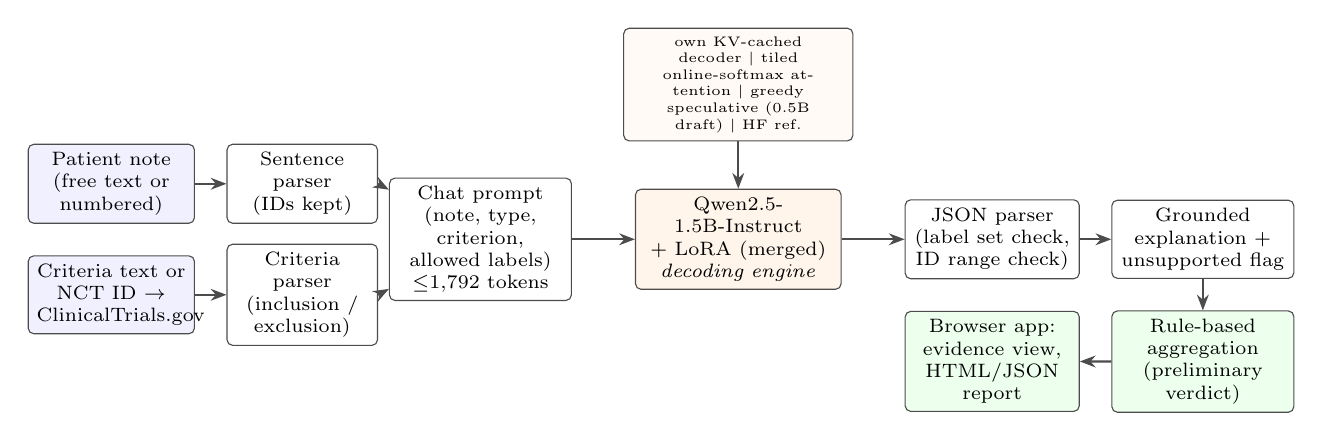
\begin{tikzpicture}[
  node distance=4mm and 4mm,
  box/.style={draw=black!70, rounded corners=2pt, align=center, font=\scriptsize, minimum height=9mm, inner sep=3pt, fill=#1},
  box/.default=white,
  arr/.style={-{Stealth[length=2mm]}, thick, black!70}]
\node[box=blue!6, text width=19mm] (note) {Patient note\\(free text or\\numbered)};
\node[box=blue!6, text width=19mm, below=of note] (crit) {Criteria text or\\NCT ID $\rightarrow$\\ClinicalTrials.gov};
\node[box, text width=17mm, right=of note] (split) {Sentence\\parser\\(IDs kept)};
\node[box, text width=17mm, right=of crit] (cparse) {Criteria parser\\(inclusion /\\exclusion)};
\node[box, text width=21mm, right=11mm of $(split)!0.5!(cparse)$] (prompt) {Chat prompt\\(note, type, criterion,\\allowed labels)\\$\le$1{,}792 tokens};
\node[box=orange!8, text width=24mm, right=8mm of prompt] (model) {Qwen2.5-1.5B-Instruct\\+ LoRA (merged)\\\textit{decoding engine}};
\node[box=orange!4, text width=27mm, above=6mm of model, font=\tiny] (eng) {own KV-cached decoder $|$ tiled\\online-softmax attention $|$ greedy\\speculative (0.5B draft) $|$ HF ref.};
\node[box, text width=20mm, right=8mm of model] (parse) {JSON parser\\(label set check,\\ID range check)};
\node[box, text width=21mm, right=of parse] (expl) {Grounded\\explanation +\\unsupported flag};
\node[box=green!7, text width=21mm, below=of expl] (agg) {Rule-based\\aggregation\\(preliminary verdict)};
\node[box=green!7, text width=20mm, below=of parse] (out) {Browser app:\\evidence view,\\HTML/JSON report};
\draw[arr] (note) -- (split); \draw[arr] (crit) -- (cparse);
\draw[arr] (split.east) -- (prompt); \draw[arr] (cparse.east) -- (prompt);
\draw[arr] (prompt) -- (model); \draw[arr] (eng) -- (model); \draw[arr] (model) -- (parse);
\draw[arr] (parse) -- (expl); \draw[arr] (expl) -- (agg); \draw[arr] (agg) -- (out);
\end{tikzpicture}
\caption{TrialMatch pipeline. Every criterion is judged independently; the patient-level verdict is a rule-based aggregation, not a learned or ground-truth label.}
\label{fig:arch}
\end{figure*}

\subsection{KV-Cached Autoregressive Decoding}\label{sec:kv}
To meet the requirement that caching be implemented rather than enabled with \texttt{use\_cache=True}, we wrote a forward pass for Qwen2-style decoders that reuses the model's weight tensors but performs every other step itself (Fig.~\ref{fig:decoder}, Algorithm~\ref{alg:kv}). For each layer, RMSNorm is followed by the $q,k,v$ projections; RoPE is applied to $q$ and $k$ at the \emph{absolute} positions $p_0,\ldots,p_0{+}T{-}1$, where $p_0$ is the current cache length. The rotated keys and the values are written into a pre-allocated cache of shape $[B, H_{kv}, \textit{capacity}, d]$. Attention then reads cache slots $[0, p_0{+}T)$; the two KV heads are repeated to serve the 12 query heads (GQA). The causal mask uses a query offset: query $i$ at absolute position $p_0{+}i$ may attend to key $j$ only if $j \le p_0{+}i$. In prefill, $p_0{=}0$ and the mask is the usual triangle; in a decode step, $T{=}1$ and every cached key is visible.

The cache stores keys \emph{after} RoPE, so cached entries never need re-rotation. It grows by doubling when its capacity is exceeded (amortised $O(1)$) and supports \texttt{crop}($n$), which simply resets the valid length; stale slots are never read. The cache costs $2\,L\,H_{kv}\,d\,b = 2\cdot28\cdot2\cdot128\cdot2 = 28{,}672$ bytes per token in 16-bit. For a 1{,}024-token prompt plus 96 generated tokens, the measured cache holds 1{,}119 positions in exactly $1{,}119\times28{,}672 = 32{,}083{,}968$ bytes. That is 1{,}119 rather than 1{,}120 because the last generated token is never fed back.

As a second, independent cached path, we drive the Hugging Face model with an explicit \texttt{DynamicCache}, passing \texttt{position\_ids}, \texttt{cache\_position} and the attention mask ourselves and asserting that the cache grows by exactly one position per step. Both cached paths are compared against two uncached references (Hugging Face and our decoder) that recompute the full sequence at every step.

\begin{figure}[t]
\centering
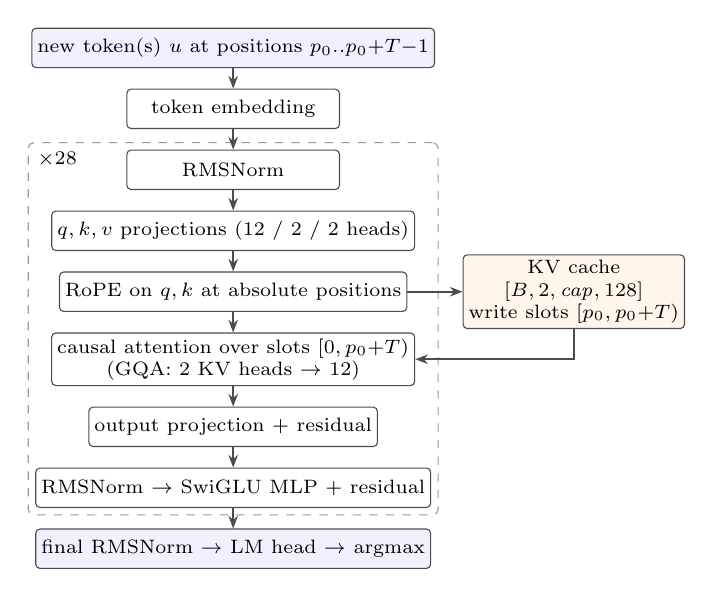
\begin{tikzpicture}[
  node distance=2.6mm,
  blk/.style={draw=black!70, rounded corners=1.5pt, align=center, font=\scriptsize, minimum width=27mm, minimum height=5mm, inner sep=2pt, fill=#1},
  blk/.default=white,
  arr/.style={-{Stealth[length=1.6mm]}, thick, black!70}]
\node[blk=blue!6] (in) {new token(s) $u$ at positions $p_0..p_0{+}T{-}1$};
\node[blk, below=of in] (emb) {token embedding};
\node[blk, below=of emb] (n1) {RMSNorm};
\node[blk, below=of n1] (qkv) {$q,k,v$ projections (12 / 2 / 2 heads)};
\node[blk, below=of qkv] (rope) {RoPE on $q,k$ at absolute positions};
\node[blk=orange!8, right=7mm of rope, minimum width=20mm] (cache) {KV cache\\$[B,2,\mathit{cap},128]$\\write slots $[p_0,p_0{+}T)$};
\node[blk, below=of rope] (att) {causal attention over slots $[0,p_0{+}T)$\\(GQA: 2 KV heads $\rightarrow$ 12)};
\node[blk, below=of att] (o) {output projection $+$ residual};
\node[blk, below=of o] (mlp) {RMSNorm $\rightarrow$ SwiGLU MLP $+$ residual};
\node[blk=blue!6, below=of mlp] (head) {final RMSNorm $\rightarrow$ LM head $\rightarrow$ argmax};
\node[draw=black!40, dashed, rounded corners=2pt, fit=(n1)(mlp), inner sep=2.5pt, label={[font=\scriptsize,anchor=north west]north west:$\times 28$}] {};
\draw[arr] (in)--(emb); \draw[arr] (emb)--(n1); \draw[arr] (n1)--(qkv); \draw[arr] (qkv)--(rope);
\draw[arr] (rope)--(att); \draw[arr] (att)--(o); \draw[arr] (o)--(mlp); \draw[arr] (mlp)--(head);
\draw[arr] (rope.east) -- (cache.west);
\draw[arr] (cache.south) |- (att.east);
\end{tikzpicture}
\caption{One decoding step of our Qwen2.5-1.5B forward pass. Keys are cached after RoPE; attention reads all cached positions plus the new ones, with the causal mask offset by $p_0$.}
\label{fig:decoder}
\end{figure}

\begin{algorithm}[t]
\caption{Greedy decoding with an explicit KV cache}\label{alg:kv}
\begin{algorithmic}[1]
\Require prompt tokens $x_{1:L}$, budget $N$, stop set $S$
\State $\mathcal{C} \gets$ allocate $K,V$ buffers of capacity $L{+}N$ per layer; $\ell\gets0$
\State $z \gets \textsc{Forward}(x_{1:L}, \mathcal{C})$ \Comment{prefill, positions $0..L{-}1$}
\State $y_1 \gets \arg\max z_L$;\; $t\gets1$
\While{$t<N$ \textbf{and} $y_t\notin S$}
  \State $z \gets \textsc{Forward}(y_t, \mathcal{C})$ \Comment{position $\ell$, attends to $0..\ell$}
  \State $y_{t+1}\gets\arg\max z$;\; $t\gets t{+}1$
\EndWhile
\Statex \textsc{Forward}$(u_{1:T},\mathcal{C})$: per layer, apply RoPE at positions $\ell..\ell{+}T{-}1$; write $k,v$ to slots $[\ell,\ell{+}T)$; attend over slots $[0,\ell{+}T)$ with causal offset $\ell$; finally $\ell\gets\ell{+}T$.
\end{algorithmic}
\end{algorithm}

\subsection{Reference and Tiled Online-Softmax Attention}\label{sec:attn}
The reference attention materialises $S=QK^\top/\sqrt{d}$, applies the offset causal mask, and normalises row-wise as $\exp(S-\max S)/\sum\exp(S-\max S)$ in FP32 (FP64 when the inputs are FP64, which provides a ground truth). The tiled kernel (Algorithm~\ref{alg:tiled}) processes a block of $B_q$ queries against key blocks of size $B_k$ and keeps, for every query row, a running maximum $m$, a running normaliser $\ell$ and an unnormalised accumulator $a$. When a new block raises the maximum to $m'$, the old state is rescaled by $\exp(m-m')$; after the last block, $o=a/\ell$. Only a $B_q\times B_k$ tile of scores is alive at any time, so memory is $O(B_qB_k + T d)$ instead of $O(T^2)$. Key blocks lying entirely in the causal future of the query block are skipped, and only diagonal blocks are masked. No fused backend is called.

\begin{algorithm}[t]
\caption{Tiled causal attention with online softmax}\label{alg:tiled}
\begin{algorithmic}[1]
\Require $Q\in\mathbb{R}^{T_q\times d}$, $K,V\in\mathbb{R}^{T_k\times d}$, offset $p_0$, blocks $B_q,B_k$
\For{each query block $Q_b$ (rows $r$)}
  \State $m\gets-\infty$, $\ell\gets0$, $a\gets\mathbf{0}$
  \For{each key block $(K_c,V_c)$ (columns $c$)}
    \If{$\min c > p_0+\max r$} \textbf{break} \Comment{causal skip}\EndIf
    \State $S\gets Q_bK_c^\top/\sqrt d$;\; $S_{ij}{\gets}{-}\infty$ if $c_j{>}p_0{+}r_i$
    \State $m'{\gets}\max(m,\mathrm{rowmax}\,S)$; $P{\gets}e^{S-m'}$; $\alpha{\gets}e^{m-m'}$
    \State $\ell\gets\alpha\ell+\mathrm{rowsum}\,P$;\; $a\gets\alpha a+PV_c$;\; $m\gets m'$
  \EndFor
  \State $O_b\gets a/\ell$
\EndFor
\end{algorithmic}
\end{algorithm}

\subsection{Greedy Speculative Decoding}\label{sec:spec}
The target (fine-tuned 1.5B) and the draft (0.5B, base or fine-tuned) both run through our decoder, so both caches are under explicit control (Algorithm~\ref{alg:spec}). Let $s$ be the committed sequence. At the start of every round the target cache holds $|s|{-}1$ positions (the last committed token has not yet been fed), and the draft cache holds at most $|s|{-}1$. The draft first consumes any committed tokens it is missing, then proposes $k$ tokens greedily. The target scores $[s_{|s|}, d_1,\ldots,d_k]$ in \emph{one} forward pass, whose $k{+}1$ argmax rows $t_0..t_k$ are its own greedy choices after each prefix. The longest prefix with $d_{i+1}=t_i$ ($a$ tokens) is accepted, and $t_a$ is appended: it is a correction if $a<k$ and a free bonus token if $a=k$. Both caches are then cropped back to $|s_{\text{new}}|{-}1$, which discards the entries of rejected draft tokens. Every committed token is therefore the target's argmax given the committed prefix, so the output must equal greedy target decoding. Stop tokens and the token budget are handled inside the accepted run. Tokenizer compatibility was checked programmatically: the vocabularies (151{,}665 entries), probe encodings and the end-of-sequence token \texttt{<|im\_end|>} are identical.

\begin{algorithm}[t]
\caption{One round of greedy speculative decoding}\label{alg:spec}
\begin{algorithmic}[1]
\Require committed $s$; target cache $\mathcal{C}_T$ ($|s|{-}1$ pos.); draft cache $\mathcal{C}_D$
\State feed $s[|\mathcal{C}_D|{:}|s|]$ to draft; propose $d_1..d_k$ greedily
\State $z\gets\textsc{Forward}_T([s_{|s|},d_1,..,d_k],\mathcal{C}_T)$;\; $t_i\gets\arg\max z_i$
\State $a\gets\max\{j: d_i=t_{i-1}\ \forall i\le j\}$
\State $s\gets s\,\Vert\,d_{1:a}\,\Vert\,t_a$ \Comment{correction or bonus token}
\State $\mathcal{C}_T.\textsc{crop}(|s|{-}1)$;\; $\mathcal{C}_D.\textsc{crop}(\min(|\mathcal{C}_D|,|s|{-}1))$
\end{algorithmic}
\end{algorithm}

\subsection{Application Workflow}
The Gradio application (Fig.~\ref{fig:app}) runs in the browser at \texttt{127.0.0.1:7860} and is started by double-clicking a launcher script that creates the environment, checks for the adapter weights and opens the browser, so no IDE or notebook is needed. A user pastes or loads a patient note, types criteria or fetches them by NCT ID from the public ClinicalTrials.gov API, and chooses a decoding engine. The application shows, for each criterion, the label, cited sentence IDs, quoted evidence, the grounded explanation and reliability flags (unsupported, parse fallback, truncation). A full-record inspector highlights the cited sentences. The preliminary verdict follows an explicit rule: \emph{likely ineligible} if any inclusion is \emph{not included} or any exclusion is \emph{excluded}; \emph{potentially eligible} if every inclusion is met or \NA\ and every exclusion is not met or \NA; otherwise \emph{undetermined---needs review}. Missing-information criteria are listed. Reports are saved as HTML and JSON with provenance (model, adapter, data type, device, decoding mode, timestamp, git commit; Fig.~\ref{fig:report}). A benchmark tab times the decoding engines live on the current input and checks that their tokens agree. Inputs are validated (empty or over-long notes, missing criteria, over-long criteria, malformed NCT IDs, network failures), and errors are reported in the interface without crashing it. An educational-prototype notice is shown on every page and in every report.

\begin{figure}[t]
\centering
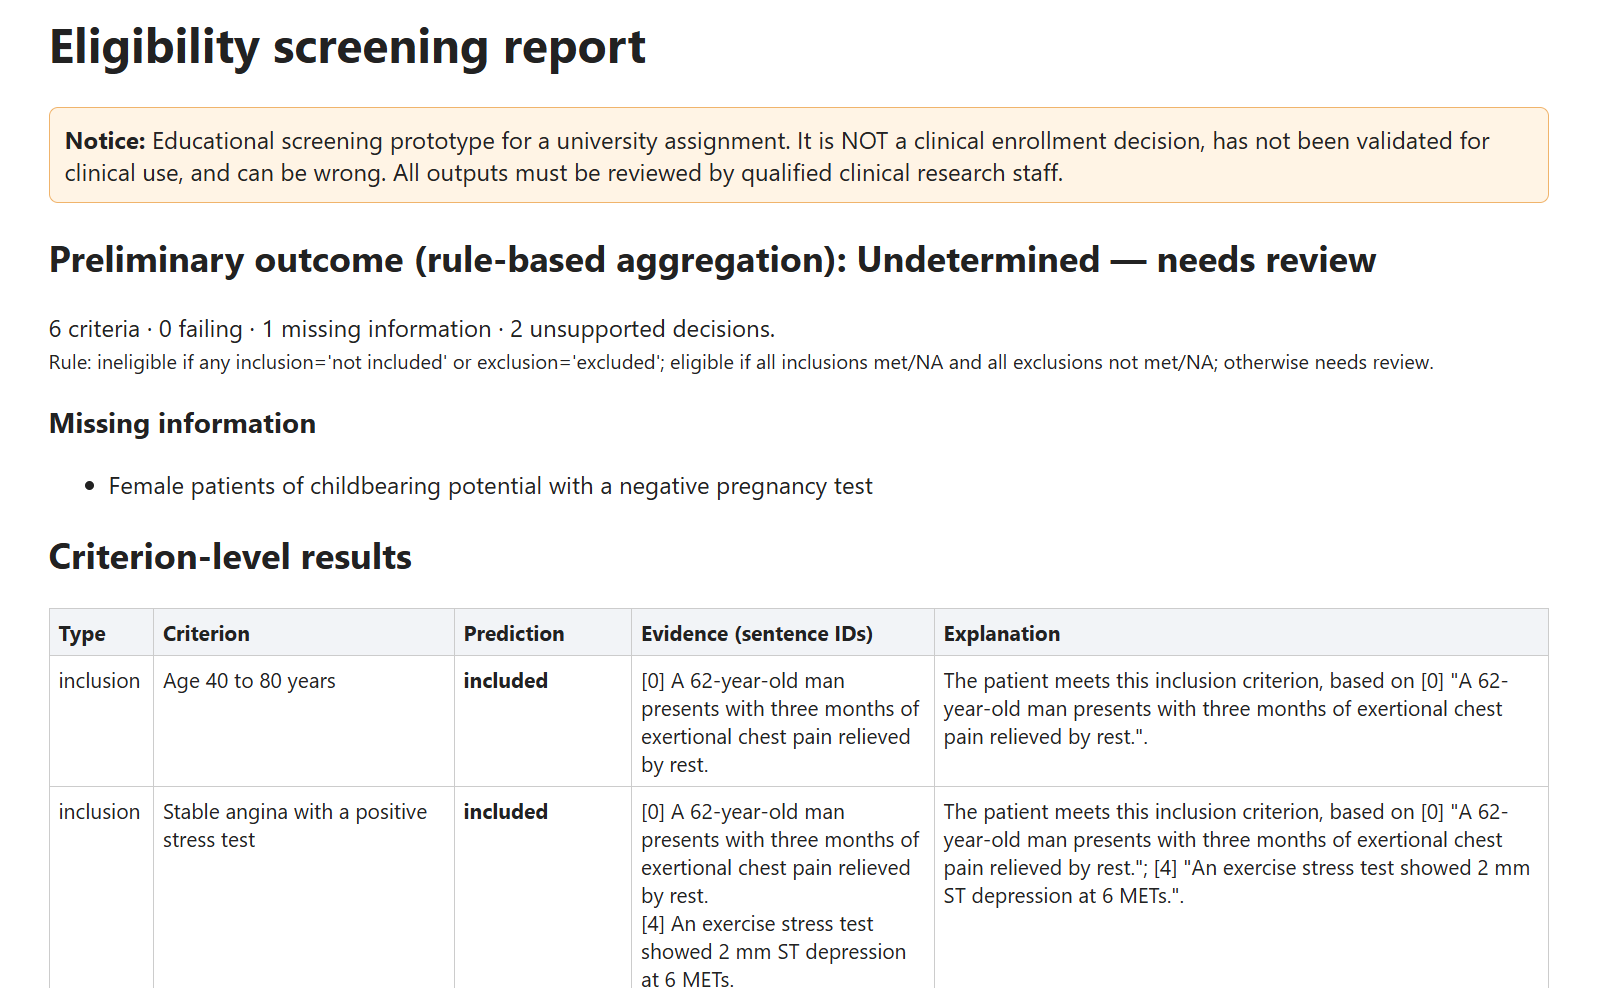
\includegraphics[width=\columnwidth]{figures/app_report.png}
\caption{Exported HTML screening report (excerpt) with the educational-prototype notice, rule-based outcome, missing-information list and criterion table quoting the cited evidence. The JSON export holds the same content plus provenance.}
\label{fig:report}
\end{figure}

% ======================================================================
\section{Experimental Setup and Metrics}
\textit{Hardware and software.} Training and benchmarks ran on a Google Colab Tesla T4 (16\,GB, compute capability 7.5) with PyTorch 2.14.1+cu130, Transformers 4.51.3 and PEFT 0.15.2; the application was also run on a CPU-only laptop.

\textit{Decoding for evaluation.} Base and fine-tuned models are evaluated on identical annotations with identical settings: greedy decoding (\texttt{do\_sample=False}, one beam, repetition penalty 1.0), at most 96 new tokens, batch size 8 with left padding, FP16. Earlier runs had silently inherited a repetition penalty from the model's default generation configuration (Section~\ref{sec:difficulties}); all reported evaluation numbers come from the corrected runs.

\textit{Classification metrics.} We report accuracy and macro-F1, overall and separately for inclusion and exclusion criteria, together with per-class precision, recall, F1 and confusion matrices. Macro-F1 averages over the labels that occur in the gold labels or the predictions of the subset being scored, so a class absent from both (\emph{excluded} on test) does not count.

\textit{Evidence metrics.} Micro precision/recall/F1 pool (record, sentence-ID) pairs over all records; a record with empty gold and empty prediction contributes nothing, and IDs predicted for an empty-gold record count as false positives. Macro P/R/F1 average per-record scores over records with non-empty gold evidence, scoring an empty prediction as 0. Records with empty gold evidence are reported separately as the rate at which the model also cites nothing.

\textit{Uncertainty and baselines.} Annotations from one patient are correlated, so 95\% confidence intervals use a patient-level bootstrap (2{,}000 resamples of the 8 patients). A majority baseline predicts the most frequent training label for each criterion type (\NEI\ for inclusion, \emph{not excluded} for exclusion).

\textit{Benchmark protocol.} All timings use \texttt{torch.cuda.synchronize()} around each measured step, one warm-up run, and the median of 3 repeats (KV cache), 5 repeats (attention) or 2 repeats (speculative). Forced-length runs ignore end-of-sequence so that every path generates exactly $N$ tokens. Decode throughput is $(N{-}1)$ divided by decode time, since the first token comes from prefill. Peak memory is \texttt{torch.cuda.max\_memory\_allocated}.

% ======================================================================
\section{Results and Discussion}

\subsection{Training Behaviour}
Fig.~\ref{fig:train} shows the answer-token loss. For the target, the training loss falls from 0.35 to about 0.07, while the validation loss reaches its minimum of 0.123 at step 80 and rises slightly to 0.131 at step 100. Selecting the best checkpoint therefore avoids the start of over-fitting on this small training set (602 examples). The draft's validation loss decreases monotonically to 0.146 (best at step 100). The final target training session took 68\,min of T4 time (draft: 25\,min) with a peak of 5.9\,GB.

\begin{figure}[t]
\centering
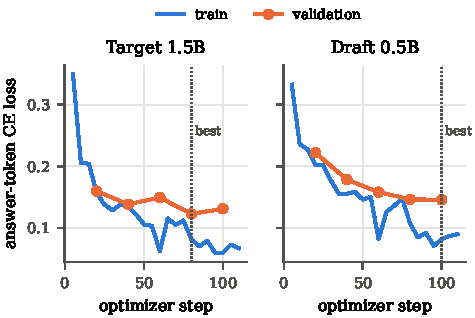
\includegraphics[width=\columnwidth]{figures/training_curves.pdf}
\caption{LoRA training and validation loss on answer tokens. The dotted line marks the checkpoint kept by validation-loss selection.}
\label{fig:train}
\end{figure}

\subsection{Criterion Classification Before and After Fine-Tuning}
Table~\ref{tab:main} compares the same model before and after fine-tuning on identical annotations. On test, accuracy rises from 0.267 to 0.733 and macro-F1 from 0.173 to 0.468. Fine-tuning fixes 100 predictions and breaks 4 (validation: 64 and 11). The patient-level bootstrap gives a test accuracy gain of $+$0.46 [0.33, 0.58] and a macro-F1 gain of $+$0.30 [0.21, 0.37]. On validation, the accuracy gain is $+$0.25 [0.11, 0.39], but the macro-F1 gain of $+$0.09 [$-$0.01, 0.20] is not statistically reliable. All outputs of both models were valid JSON with an allowed label.

The base model behaves very differently on the two splits (0.461 on validation vs.\ 0.267 on test), which shows how much eight patients can vary. Its dominant error is semantic: it labels 60 of 91 test criteria that are \emph{not excluded} as \emph{excluded} (Fig.~\ref{fig:cm}), apparently reading ``excluded'' as ``the criterion is ruled out''. It also cites evidence for every decision, with precision 0.077. Fine-tuning teaches the dataset's label semantics and output conventions.

\begin{table}[t]
\caption{Base vs.\ fine-tuned Qwen2.5-1.5B (greedy, FP16)}
\label{tab:main}
\centering
\footnotesize
\setlength{\tabcolsep}{2.6pt}
\begin{tabular}{llcccccc}
\toprule
Split & Model & Acc & M-F1 & Incl.\ acc & Excl.\ acc & Ev.\ $\mu$F1 & Ev.\ MF1\\
\midrule
\multirow{3}{*}{Val} & Majority & 0.621 & 0.215 & 0.409 & 0.721 & -- & --\\
 & Base & 0.461 & 0.263 & 0.545 & 0.421 & 0.122 & 0.211\\
 & Fine-tuned & \textbf{0.718} & \textbf{0.349} & \textbf{0.712} & \textbf{0.721} & \textbf{0.534} & \textbf{0.577}\\
\midrule
\multirow{3}{*}{Test} & Majority & 0.626 & 0.272 & 0.507 & 0.695 & -- & --\\
 & Base & 0.267 & 0.173 & 0.360 & 0.214 & 0.136 & 0.317\\
 & Fine-tuned & \textbf{0.733} & \textbf{0.468} & \textbf{0.800} & \textbf{0.695} & \textbf{0.601} & \textbf{0.569}\\
\bottomrule
\end{tabular}
\\[2pt]
\parbox{\columnwidth}{\scriptsize M-F1: macro-F1; Ev.\ $\mu$F1 / MF1: evidence micro / macro F1. Majority: \NEI\ for inclusion, \emph{not excluded} for exclusion (from training labels).}
\end{table}

\textit{Comparison with the majority baseline.} The fine-tuned model beats the trivial baseline by 0.10--0.11 accuracy and 0.13--0.20 macro-F1, but Table~\ref{tab:main} shows where that gain comes from. On exclusion criteria its accuracy equals the baseline exactly (0.695 on test, 0.721 on validation): it predicts \emph{not excluded} for \emph{every} exclusion criterion, 131 of 131 on test and 140 of 140 on validation. All of the real gain is on inclusion criteria (0.507 $\rightarrow$ 0.800 on test), where the model reliably separates \emph{included} from \NEI.

\begin{figure}[t]
\centering
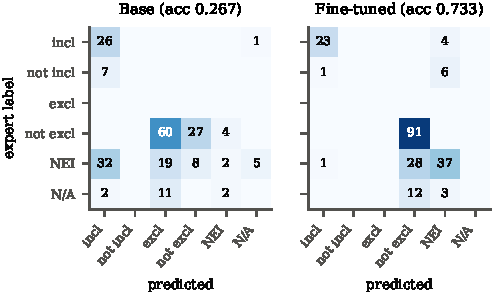
\includegraphics[width=\columnwidth]{figures/confusion_test.pdf}
\caption{Test confusion matrices (rows: expert label; NEI: not enough information; N/A: not applicable). The base model inverts exclusion polarity; the fine-tuned model collapses all exclusion criteria onto \emph{not excluded}.}
\label{fig:cm}
\end{figure}

\subsection{Per-Class Results}
Table~\ref{tab:perclass} reports per-class results on the test set (validation follows the same pattern). \emph{Included} reaches F1 0.885 and \NEI\ 0.638, while \emph{not included} (7 test cases), \emph{not applicable} (15) and \emph{excluded} (none in test; 2 in validation) are never predicted correctly; on both splits the model never outputs them at all. These classes make up only 2.2\%, 4.7\% and 1.3\% of the training labels, so the cross-entropy objective is minimised by predicting the frequent neighbouring class instead. This class collapse is why macro-F1 stays below 0.5 while accuracy exceeds 0.7.

\begin{table}[t]
\caption{Per-class results of the fine-tuned model on test}
\label{tab:perclass}
\centering
\footnotesize
\begin{tabular}{lcccc}
\toprule
Class & Precision & Recall & F1 & Support\\
\midrule
included & 0.920 & 0.852 & 0.885 & 27\\
not included & 0.000 & 0.000 & 0.000 & 7\\
excluded & -- & -- & -- & 0\\
not excluded & 0.695 & 1.000 & 0.820 & 91\\
not enough information & 0.740 & 0.561 & 0.638 & 66\\
not applicable & 0.000 & 0.000 & 0.000 & 15\\
\bottomrule
\end{tabular}
\end{table}

\subsection{Evidence Sentence Localisation}
Table~\ref{tab:evidence} summarises evidence retrieval. The base model cites sentences indiscriminately, with high recall (0.564) but precision 0.077, and on only 4\% of empty-gold records does it correctly cite nothing. The fine-tuned model balances precision (0.586) and recall (0.617) for a micro-F1 of 0.601, and it leaves 91.7\% of empty-gold records empty, matching the annotators' practice. Evidence is better on inclusion (micro-F1 0.671) than on exclusion (0.415) criteria, consistent with the label results.

\begin{table}[t]
\caption{Evidence sentence retrieval on test}
\label{tab:evidence}
\centering
\footnotesize
\setlength{\tabcolsep}{3pt}
\begin{tabular}{lcccccc}
\toprule
 & \multicolumn{3}{c}{Micro (all 206)} & \multicolumn{2}{c}{Macro (61 non-empty)} & Empty gold\\
\cmidrule(lr){2-4}\cmidrule(lr){5-6}
Model & P & R & F1 & P & F1 & correct-empty\\
\midrule
Base & 0.077 & 0.564 & 0.136 & 0.273 & 0.317 & 6/145\\
Fine-tuned & 0.586 & 0.617 & 0.601 & 0.563 & 0.569 & 133/145\\
\bottomrule
\end{tabular}
\end{table}

\subsection{Error Analysis}
Each wrong label was assigned exactly one error type (Table~\ref{tab:errors}). Fine-tuning almost eliminates polarity errors (67 $\rightarrow$ 1). The largest remaining type is \emph{decision without information}: the experts judged a criterion undecidable and the model nevertheless answered \emph{not excluded}. Table~\ref{tab:errors} also checks the \emph{unsupported} flag (decisive label, no cited sentence). The experts themselves give 84 of their 125 decisive test labels (67\%) with no evidence, typically \emph{not excluded} for a condition the note never mentions. The model's rate is 121/156 (78\%), and 82 of those predictions have the correct label. The flag therefore marks the annotation convention far more often than model failures: it is a cue for human review, not an error count.

\begin{table}[t]
\caption{Label error types on test (each wrong label counted once)}
\label{tab:errors}
\centering
\footnotesize
\setlength{\tabcolsep}{3pt}
\begin{tabular}{p{4.6cm}cc}
\toprule
Error type (gold $\rightarrow$ predicted) & Base & FT\\
\midrule
Polarity (decisive $\rightarrow$ opposite decisive) & 67 & 1\\
Decision without information (\NEI\ $\rightarrow$ decisive) & 59 & 29\\
Applicability (\NA\ involved) & 21 & 15\\
Missed information (decisive $\rightarrow$ \NEI) & 4 & 10\\
\midrule
Total wrong labels & 151 & 55\\
\midrule
Decisive with no cited evidence: experts & \multicolumn{2}{c}{84/125}\\
Decisive with no cited evidence: model (correct label) & 0/192 & 121/156 (82)\\
\bottomrule
\end{tabular}
\end{table}

The following nine test errors (all from patients the model never saw) illustrate the failure modes. Sentence numbers refer to the patient's note.

\begin{enumerate}
\item \textbf{Missed information, inference by context} (ann.\ 161). Criterion: ``Patients undergoing elective carotid endarterectomy''; the patient had a cardiac catheterisation with a femoral complication. Expert: \emph{not included}; model: \NEI. The experts infer that a patient described in full who is not undergoing the procedure does not qualify; the model treats the absence as unknown. The same pattern explains six of the seven \emph{not included} errors.
\item \textbf{Polarity through lexical overlap} (ann.\ 164). ``Surgical lower-limb revascularisation'': the model answered \emph{included}, citing [0] (catheterisation via the femoral artery) and [2] (pulsatile groin mass). It matched vascular vocabulary rather than the procedure, which is the only polarity error left after fine-tuning.
\item \textbf{Decision without information} (ann.\ 169). ``Pre-operative eGFR $<$ 30'': expert \NEI, model \emph{not excluded} with no evidence. No renal function is reported, so the model treated absent evidence as proof of a negative, exactly what the task forbids. This is the most frequent error (29 cases), and the training labels encourage it, since unmentioned exclusions are usually labelled \emph{not excluded}.
\item \textbf{Decision without information, global criterion} (ann.\ 193). ``Patients were moribund'': the experts cite all five sentences and answer \NEI; the model answers \emph{not excluded} with no evidence. Holistic judgements of the whole record are beyond what the model learned from sentence-level evidence.
\item \textbf{Applicability} (ann.\ 165). ``Pregnancy'' for a 67-year-old woman: expert \NA, model \emph{not excluded}. The two answers mean the same in practice; the boundary between \NA\ and a negated criterion is not consistent in the annotations, and the model, which never predicts \NA, defaults to the frequent class (12 of 15 \NA\ errors).
\item \textbf{Applicability with explicit evidence} (ann.\ 422). ``If female, using birth control'': the expert cites [3] (no sexual partners) and answers \NA; the model answers \NEI\ without evidence. Recognising that a conditional criterion does not apply needs a reasoning step the model did not learn from 28 \NA\ training examples.
\item \textbf{Right evidence, missed clinical inference} (ann.\ 185). ``Diagnosed with shock, ARDS, or both'': the model cites [2] (pale, tachypnoeic, tachycardic) and [3] (BP 80/60), the expert's evidence plus one sentence, yet answers \NEI. It found the facts but did not infer shock from hypotension with tachycardia.
\item \textbf{Missed implicit numeric threshold} (ann.\ 186). ``Heart rate of at least 90/min'': expert \emph{included} from [2] (``tachycardic'', i.e.\ $>$100/min); the model cites the blood-pressure sentence and answers \NEI. Turning a qualitative finding into a numeric bound needs clinical knowledge the 1.5B model lacks.
\item \textbf{Same evidence, contradictory label} (ann.\ 762). ``Sore throat \ldots\ together with at least 2 of the following clinical signs:'' cites the same sentence [0] as the expert but answers \emph{included} where the expert says \NEI. The criterion text in the dataset is cut off before the list of signs, so the condition cannot be checked; the model over-commits on an incomplete criterion.
\end{enumerate}

An unseen case typed into the application shows the same weakness in numeric reasoning. For a diabetic patient with ``HbA1c is 8.4\%'' and the criterion ``HbA1c between 7.5\% and 10.5\%'', the model cited the correct sentence but answered \NEI\ instead of \emph{included}. In summary, the dominant failures are (i) collapse onto frequent labels, (ii) treating absence as a negative for exclusion criteria, and (iii) clinical or numeric inference beyond surface matching. Evidence extraction is comparatively good: when the model cites a sentence it is usually relevant.

\subsection{KV-Cached Decoding}
\textit{Correctness.} Table~\ref{tab:kv} summarises seven cases: one real prompt that stops at end-of-sequence, and forced generation with $L\in\{128,512,1024\}$ input and $N\in\{32,96\}$ output tokens. In BF16, all four paths agree on five cases. In the $L{=}128$ cases, \emph{both} cached paths (ours and Hugging Face's) diverge from the uncached reference at token 27, where the reference's top two logits are 22.0 and 21.875. BF16 has 8 significand bits, so between 16 and 32 the representable values are spaced 0.125 apart: the two candidates are tied to within one rounding step, and a different reduction order in the cached computation flips the argmax. That Hugging Face's cache flips identically rules out a bug specific to our cache. Re-running in FP32 makes all paths agree in every case, and our cached logits match a full Hugging Face forward pass to within $5.3\times10^{-5}$ (mean $5.6\times10^{-6}$), against 0.31 in BF16. The cache logic is therefore exact; the BF16 differences are numerical ties.

\begin{table}[t]
\caption{KV-cache benchmark (BF16, $N{=}96$ output tokens): decode tokens/s and peak memory}
\label{tab:kv}
\centering
\footnotesize
\setlength{\tabcolsep}{2.6pt}
\begin{tabular}{lcccccc}
\toprule
 & \multicolumn{2}{c}{$L{=}128$} & \multicolumn{2}{c}{$L{=}512$} & \multicolumn{2}{c}{$L{=}1024$}\\
\cmidrule(lr){2-3}\cmidrule(lr){4-5}\cmidrule(lr){6-7}
Path & tok/s & MiB & tok/s & MiB & tok/s & MiB\\
\midrule
HF uncached & 3.46 & 3083 & 1.21 & 3307 & 0.62 & 3605\\
HF + DynamicCache & 23.8 & 2998 & 22.3 & 3128 & 19.9 & 3302\\
Ours uncached & 4.04 & 2971 & 1.43 & 3020 & 0.72 & 3138\\
Ours + own cache & 22.6 & 2969 & 23.9 & 3021 & 23.4 & 3141\\
\midrule
\multicolumn{7}{l}{Token agreement with HF uncached: 5/7 cases (BF16), 3/3 (FP32);}\\
\multicolumn{7}{l}{BF16 mismatch at $L{=}128$, step 27, top-2 logit margin 0.125.}\\
\bottomrule
\end{tabular}
\end{table}

\textit{Performance.} Fig.~\ref{fig:kv} and Table~\ref{tab:kv} show the expected asymptotics. Without a cache, every step reprocesses the whole sequence, so decode throughput falls roughly in proportion to length (3.5 $\rightarrow$ 0.62 tokens/s for Hugging Face). With a cache, each step processes one token and throughput stays almost constant (about 20--24 tokens/s). At $L{=}1024$, caching raises decode throughput 32$\times$ (per-step latency 41\,ms vs.\ 1{,}585\,ms). Prefill costs the same with or without a cache (1.27--1.49\,s at $L{=}1024$). Our uncached decoder uses less memory than Hugging Face's because it projects only the last position onto the 151{,}936-word vocabulary, whereas Hugging Face computes logits for every position (about 0.3\,GB at 1k tokens); this difference has nothing to do with caching. All absolute speeds are depressed by emulated BF16: in FP32, our cached decoder reaches 30.6 tokens/s at $L{=}128$.

\begin{figure}[t]
\centering
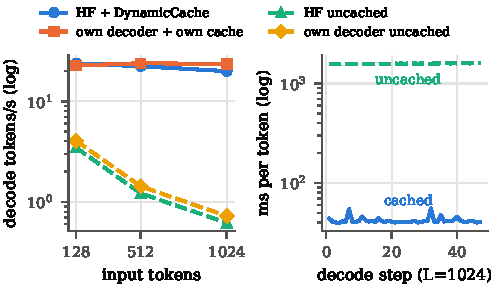
\includegraphics[width=\columnwidth]{figures/kvcache.pdf}
\caption{Left: decode throughput vs.\ input length ($N{=}96$, log scale). Right: per-step latency at $L{=}1024$ for cached and uncached Hugging Face decoding.}
\label{fig:kv}
\end{figure}

\subsection{Tiled Online-Softmax Attention}
\textit{Correctness.} Table~\ref{tab:attn} covers eight shapes in FP32 and FP16, including a single element, sizes not divisible by the block size, a cached decode step (one query at offset 256), a speculative verification chunk (five queries at offset 295), and a single-tile case. Every case passes: the maximum tiled-vs-reference error is $8.0\times10^{-6}$ in FP32 and $9.8\times10^{-4}$ in FP16, which is one FP16 unit in the last place at magnitude~1. Against the FP64 ground truth, tiled, reference and SDPA errors are all of the same order, so tiling adds no measurable error. Changing future keys and values leaves earlier outputs unchanged (no causal leakage), and inputs with $|\text{scores}|$ in the tens of thousands stay finite with zero error, confirming the stability of the running maximum. The block counts match causal skipping exactly: for $T{=}64$ with 16$\times$16 tiles, 10 of 16 tiles are computed.

\begin{table}[t]
\caption{Attention correctness (max / mean absolute error vs.\ reference)}
\label{tab:attn}
\centering
\footnotesize
\setlength{\tabcolsep}{3pt}
\resizebox{\columnwidth}{!}{%
\begin{tabular}{lccc}
\toprule
 & Tiled vs ref (max) & Tiled vs ref (mean) & Tolerance\\
\midrule
FP32, 8 shapes & $7.96\times10^{-6}$ & $\le3.6\times10^{-7}$ & $10^{-5}$\\
FP16, 8 shapes & $9.77\times10^{-4}$ & $\le3.6\times10^{-7}$ & $10^{-2}$\\
\midrule
\multicolumn{4}{l}{vs.\ FP64 (FP32): tiled $6.7\times10^{-6}$, reference $5.4\times10^{-6}$, SDPA $5.6\times10^{-6}$}\\
\multicolumn{4}{l}{Full model, 48 tokens: identical tokens with SDPA, reference, tiled}\\
\bottomrule
\end{tabular}}
\end{table}

\textit{Performance.} Fig.~\ref{fig:attn} shows that the reference implementation's extra memory grows quadratically, reaching 2{,}304\,MiB at $T{=}4096$: the FP32 score matrix ($12\cdot T^2\cdot4$\,B $=$ 768\,MiB) is held about three times, as scores, masked scores and exponentials. The tiled kernel grows linearly and uses 40.5\,MiB with 128$\times$128 tiles, 57$\times$ less. It is, however, slower than the reference (252\,ms vs.\ 62\,ms) and 59$\times$ slower than PyTorch's fused SDPA (4.2\,ms, 12\,MiB). This is expected for an educational kernel: each tile issues several small, separately launched GPU operations from a Python loop, so time scales with the number of tiles. Quadrupling the tile area reduces the time 3.9$\times$, almost exactly the 4$\times$ fewer iterations, which confirms that the kernel is overhead-bound. A fused kernel performs the same recurrence inside on-chip SRAM in one launch~\cite{dao2022flash}. Inside the full model (384-token prompt, 48 tokens, BF16) the three kernels generate identical tokens at 25.1 (SDPA), 17.6 (reference) and 7.3 (tiled) tokens/s. The tiled kernel should therefore be presented as a correct, memory-saving implementation, not a faster one.

\begin{figure}[t]
\centering
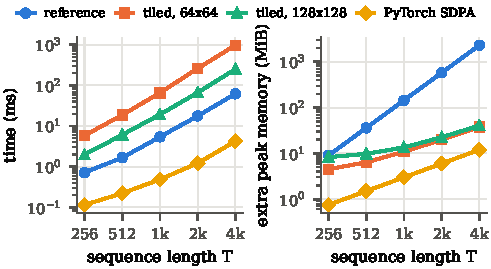
\includegraphics[width=\columnwidth]{figures/attention.pdf}
\caption{Causal self-attention ($H{=}12$, $d{=}128$, FP16, T4): time and extra peak memory vs.\ sequence length (log--log).}
\label{fig:attn}
\end{figure}

\subsection{Greedy Speculative Decoding}
\textit{Correctness.} Three runs establish exactness (Table~\ref{tab:spec}). (i)~In FP32 with the fine-tuned target and both drafts, speculative decoding matched greedy target decoding on all 72 natural-EOS runs (12 prompts $\times$ 2 drafts $\times$ $k\in\{2,4,6\}$). (ii)~In FP32 with the base target and base draft, after the repetition-penalty fix, all 72 runs matched in both the natural and forced 128-token settings, and Hugging Face's \texttt{generate} and assisted generation also matched our greedy decoder on all 12 prompts. (iii)~In BF16, natural-EOS runs matched on 72/72, but forced 128-token runs matched on only 47/72. Every first mismatch lies beyond the point where the same prompt's natural answer ended (e.g.\ token 21 vs.\ a 14-token answer), i.e.\ in low-confidence forced filler. Within a prompt, the first mismatch often occurs at the same position for both drafts and every $k$ (e.g.\ token 31 in all six runs of one prompt), whereas a bug in proposal handling would depend on what the draft proposed. Together with the FP32 results, this attributes the mismatches to BF16 ties in the target's multi-token verification pass, the same mechanism as in the KV-cache test.

\begin{table}[t]
\caption{Speculative decoding (fine-tuned 1.5B target, BF16, natural EOS, 12 prompts)}
\label{tab:spec}
\centering
\footnotesize
\setlength{\tabcolsep}{3pt}
\begin{tabular}{llccccc}
\toprule
Draft & $k$ & Accept & Tok/fwd & Tok/s & Speed-up & Equal\\
\midrule
-- (greedy target) & -- & -- & 1.00 & 14.1 & 1.00 & --\\
\midrule
\multirow{3}{*}{Base 0.5B} & 2 & 0.746 & 2.41 & 9.2 & 0.65 & 12/12\\
 & 4 & 0.708 & 3.27 & 9.3 & 0.66 & 12/12\\
 & 6 & 0.640 & 3.93 & 9.0 & 0.64 & 12/12\\
\midrule
\multirow{3}{*}{Fine-tuned 0.5B} & 2 & 0.969 & 2.75 & 10.1 & 0.72 & 12/12\\
 & 4 & 0.936 & 4.36 & 10.7 & 0.76 & 12/12\\
 & 6 & 0.932 & 5.85 & 10.9 & 0.77 & 12/12\\
\midrule
\multicolumn{2}{l}{HF assisted (base / FT)} & -- & -- & 9.8 / 11.4 & 0.81 / 0.94 & --\\
\bottomrule
\end{tabular}
\\[2pt]
\parbox{\columnwidth}{\scriptsize Tok/fwd: committed tokens per target forward. Peak memory: 4{,}908\,MiB greedy vs.\ 4{,}914\,MiB speculative (both drafts resident). FP32 runs: 72/72 equal (fine-tuned target), 72/72 equal in both settings (base target).}
\end{table}

\textit{Acceptance and speed.} Fine-tuning the draft on the same data raises acceptance from 0.64--0.75 to 0.93--0.97, because the draft learns the JSON format and label vocabulary (Fig.~\ref{fig:spec}). The measured tokens per target forward agree with theory: with acceptance $\alpha$ and $k$ drafts, the expected tokens per round are $(1-\alpha^{k+1})/(1-\alpha)$, i.e.\ 4.40 for $\alpha{=}0.936$, $k{=}4$, against 4.36 measured. Yet every configuration is slower than greedy decoding, with a best of 0.77$\times$. Writing the cost of one draft step as $c$ target steps, the speed-up is about $E[\text{tokens}]/(kc+1)$; solving with our measurements gives $c\approx1.1$--$1.2$. That is, a 0.5B draft step costs about as much as a 1.5B target step. At batch size 1 on a T4, both models are limited by fixed per-layer costs (kernel launches and Python dispatch in our decoder) rather than by arithmetic, and the draft has 24 layers against the target's 28. For a speed-up at $k{=}4$ the draft would need $c<0.84$, which in practice requires a much larger target-to-draft size ratio (e.g.\ a 7B target) or fused kernels. Hugging Face's optimised assisted generation is also slower than greedy on this setup (0.81--0.94$\times$), confirming that the slowdown comes from the hardware regime rather than our implementation. Speculative decoding is therefore reported as correct, with high acceptance, but without an end-to-end speed-up here. Memory rises by only 6\,MiB of cache over greedy decoding, since both models' weights are resident in either case.

\begin{figure}[t]
\centering
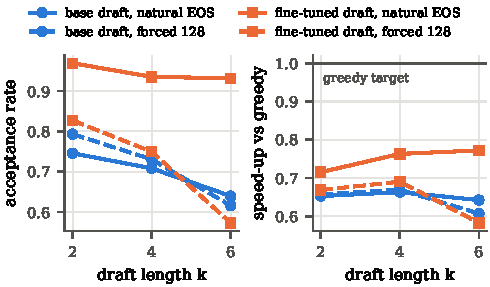
\includegraphics[width=\columnwidth]{figures/speculative.pdf}
\caption{Draft acceptance rate (left) and speed-up over greedy target decoding (right) vs.\ draft length (BF16, T4). All speed-ups are below 1.}
\label{fig:spec}
\end{figure}

\subsection{Design Alternatives and Observed Difficulties}\label{sec:difficulties}
Table~\ref{tab:design} lists the main alternatives and the evidence behind each choice. Three difficulties changed the project:
\begin{enumerate}
\item \textbf{Emulated BF16.} PyTorch reports BF16 as supported on the T4, so it was selected automatically. FP32 then ran faster than BF16 (30.6 vs.\ 25.4 cached tokens/s at $L{=}128$; 18.3 vs.\ 14.1 tokens/s for greedy target decoding in the speculative benchmark), and 1{,}024-token prefill took 1.5\,s, far slower than native FP16. The device check now selects BF16 only on GPUs with compute capability $\ge 8$; evaluation was re-run in FP16.
\item \textbf{Hidden repetition penalty.} Hugging Face \texttt{generate} matched our greedy decoder on only 8/12 prompts, \emph{even in FP32}, which ruled out rounding. The cause was the repetition penalty in Qwen2.5-Instruct's default generation configuration: \texttt{do\_sample=False} disables sampling but not the penalty. Because the penalty also applies to prompt tokens, which contain every label word, it mainly perturbed the less confident base model. After the penalty was set to 1.0 explicitly, agreement became 12/12 and all evaluations were re-run, which changed base-model test accuracy from 0.383 to 0.267 while the fine-tuned model was almost unchanged (0.728 $\rightarrow$ 0.733).
\item \textbf{Parameter counting with tied embeddings} overstated the candidates' sizes until the meta-device model was explicitly tied (Table~\ref{tab:models}).
\end{enumerate}

\begin{table}[t]
\caption{Design alternatives and evidence for the final choice}
\label{tab:design}
\centering
\scriptsize
\setlength{\tabcolsep}{2.5pt}
\begin{tabular}{p{1.35cm}p{2.85cm}p{3.75cm}}
\toprule
Decision & Alternatives & Choice and evidence\\
\midrule
Target model & Qwen2.5-3B, SmolLM2-1.7B, Llama-3.2-1B & Qwen2.5-1.5B: licence, GQA cache, same-tokenizer draft, fits T4 (5.9\,GB peak)\\
Adaptation & full fine-tuning, QLoRA & LoRA r16 on all projections: 1.2\% trainable, no quantisation error\\
Loss & full-sequence & answer-only (prompt masked)\\
Checkpoint & last step & best validation loss (step 80; val.\ loss rises after)\\
Explanation & free-text generation & grounded template (no supervision available; cannot invent facts)\\
Draft & base 0.5B & fine-tuned 0.5B: acceptance 0.71 $\rightarrow$ 0.94 ($k{=}4$)\\
Draft length & $k\in\{2,4,6\}$ & $k{=}4$--6 best speed-up (0.76--0.77)\\
Tile size & 64$\times$64, 128$\times$128 & 128: 3.9$\times$ faster, similar memory\\
Precision & BF16, FP16, FP32 & FP16 on T4 (BF16 emulated); FP32 for exactness tests\\
Decoding & HF default config & explicit greedy, repetition penalty 1.0\\
\bottomrule
\end{tabular}
\\[2pt]
\parbox{\columnwidth}{\scriptsize Evidence-first output order and the grounded explanation template were design choices that were not ablated.}
\end{table}

\subsection{Browser Application}
Fig.~\ref{fig:app} shows the application on a CPU-only laptop (FP32), where a criterion takes 11--18\,s and the first call about 29\,s because of one-off initialisation. For the demonstration case (seven-sentence chest-pain note, six criteria), the model includes age and stable angina with cited evidence (sentences 0 and 4), returns \NEI\ for the pregnancy-test criterion of this male patient, which an expert would arguably label \NA, and excludes no criterion. The rule therefore yields \emph{undetermined---needs review}. Two exclusions carry \emph{unsupported} flags: ejection fraction, which the note never mentions, and oral anticoagulants, where the model missed the explicit sentence ``He is not taking any anticoagulants'', an evidence-recall failure. The live benchmark tab reports, for instance, identical tokens for the own-cache and tiled engines, with the tiled engine 1.3$\times$ slower on CPU. This mirrors the GPU results inside the deployed system.

\begin{figure*}[t]
\centering
\begin{minipage}[t]{0.49\textwidth}\centering
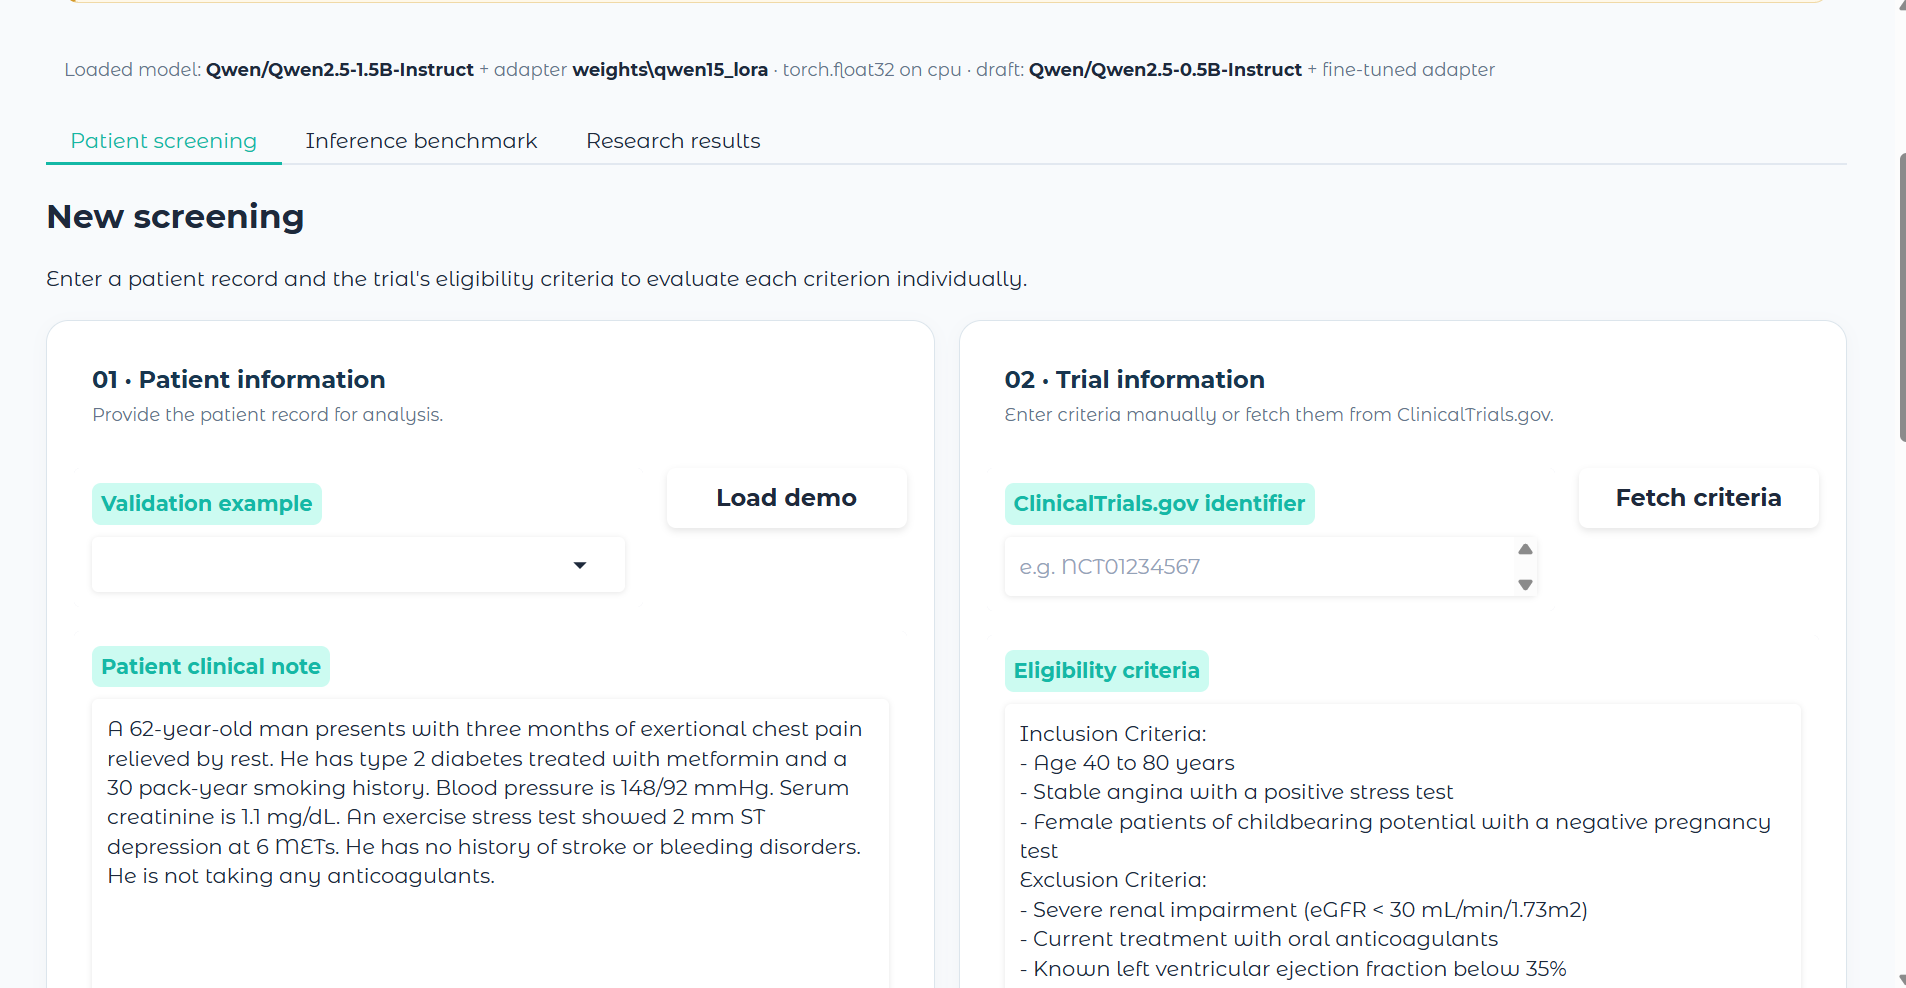
\includegraphics[width=\linewidth]{figures/app_input.png}\\[-1pt]{\footnotesize (a) Input: note, criteria, NCT fetch, engine selection}
\end{minipage}\hfill
\begin{minipage}[t]{0.49\textwidth}\centering
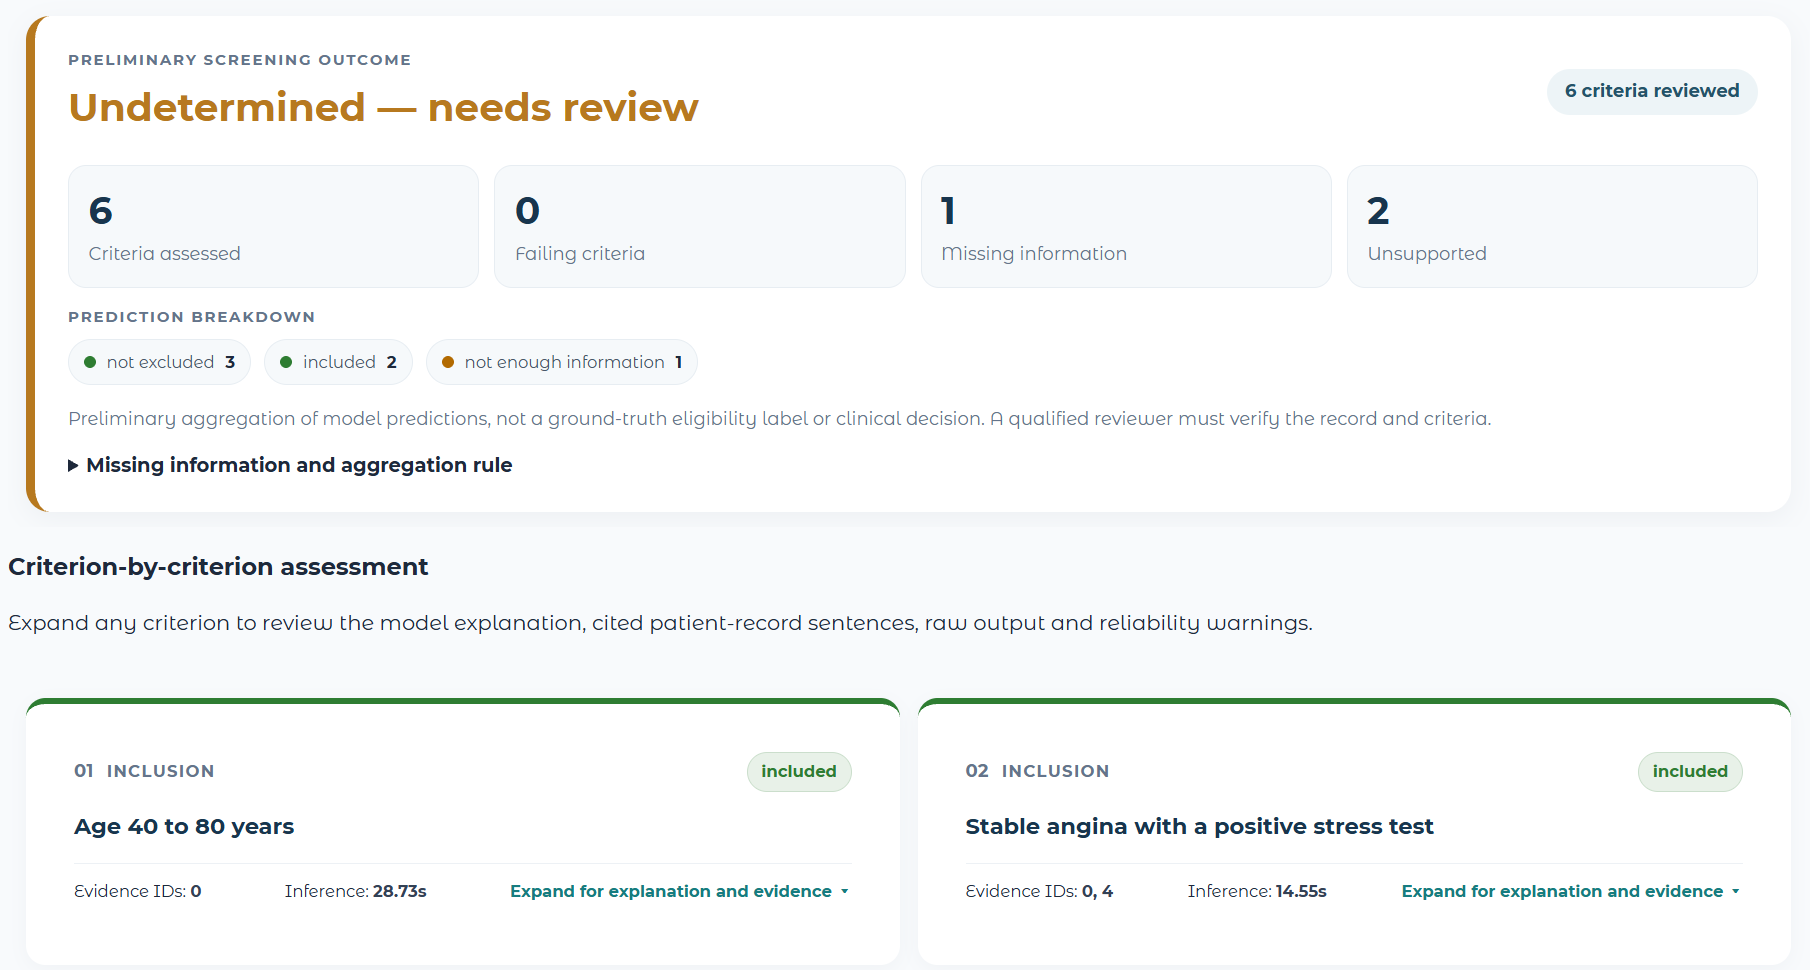
\includegraphics[width=\linewidth]{figures/app_verdict.png}\\[-1pt]{\footnotesize (b) Rule-based verdict, label breakdown, criterion cards}
\end{minipage}\\[6pt]
\begin{minipage}[t]{0.49\textwidth}\centering
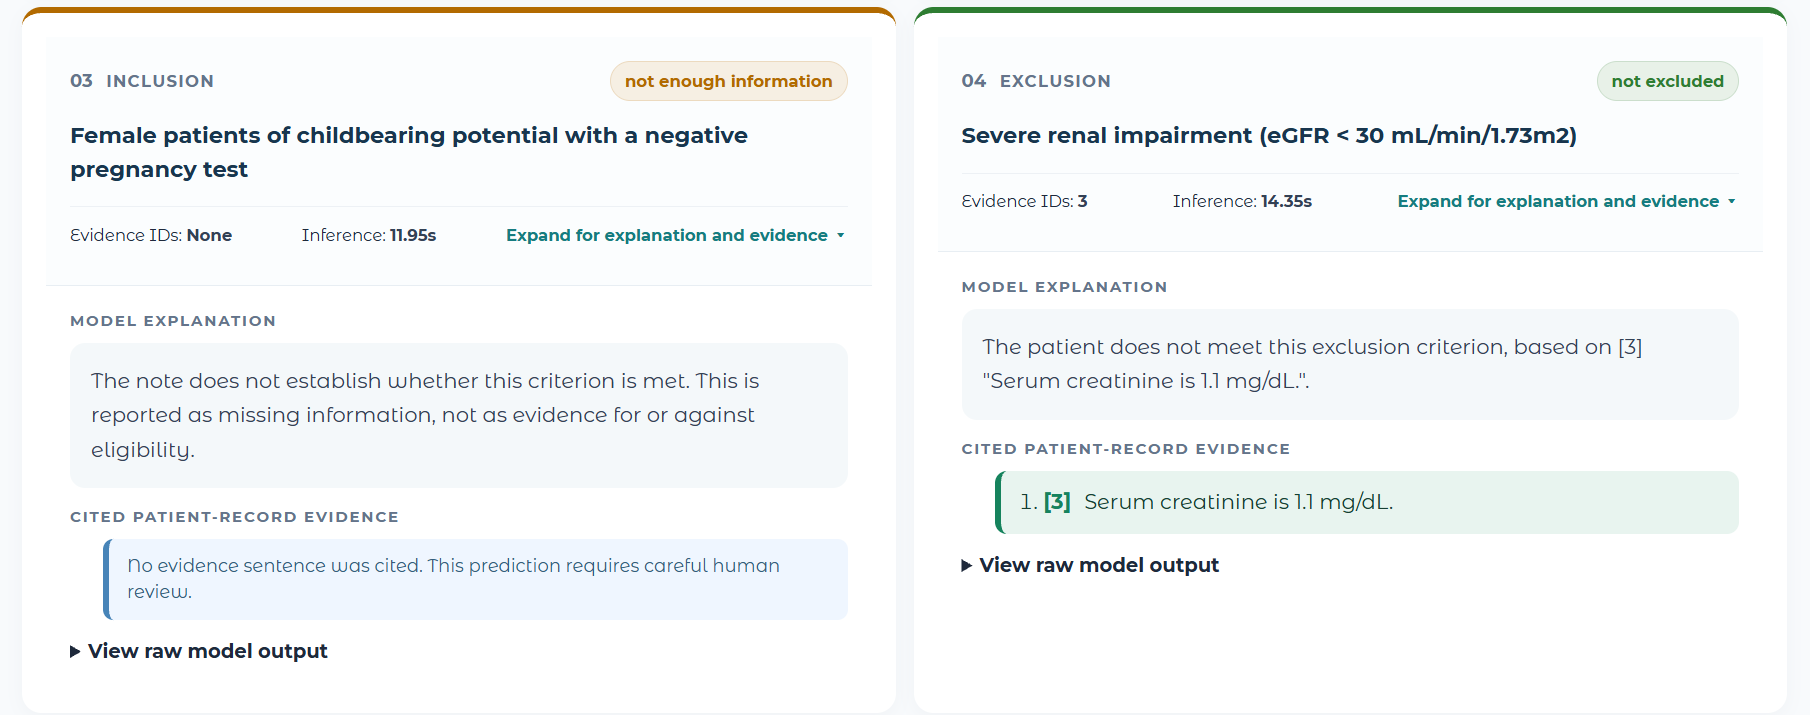
\includegraphics[width=\linewidth]{figures/app_cards.png}\\[-1pt]{\footnotesize (c) Expanded cards: grounded explanation, cited evidence, flags}
\end{minipage}\hfill
\begin{minipage}[t]{0.49\textwidth}\centering
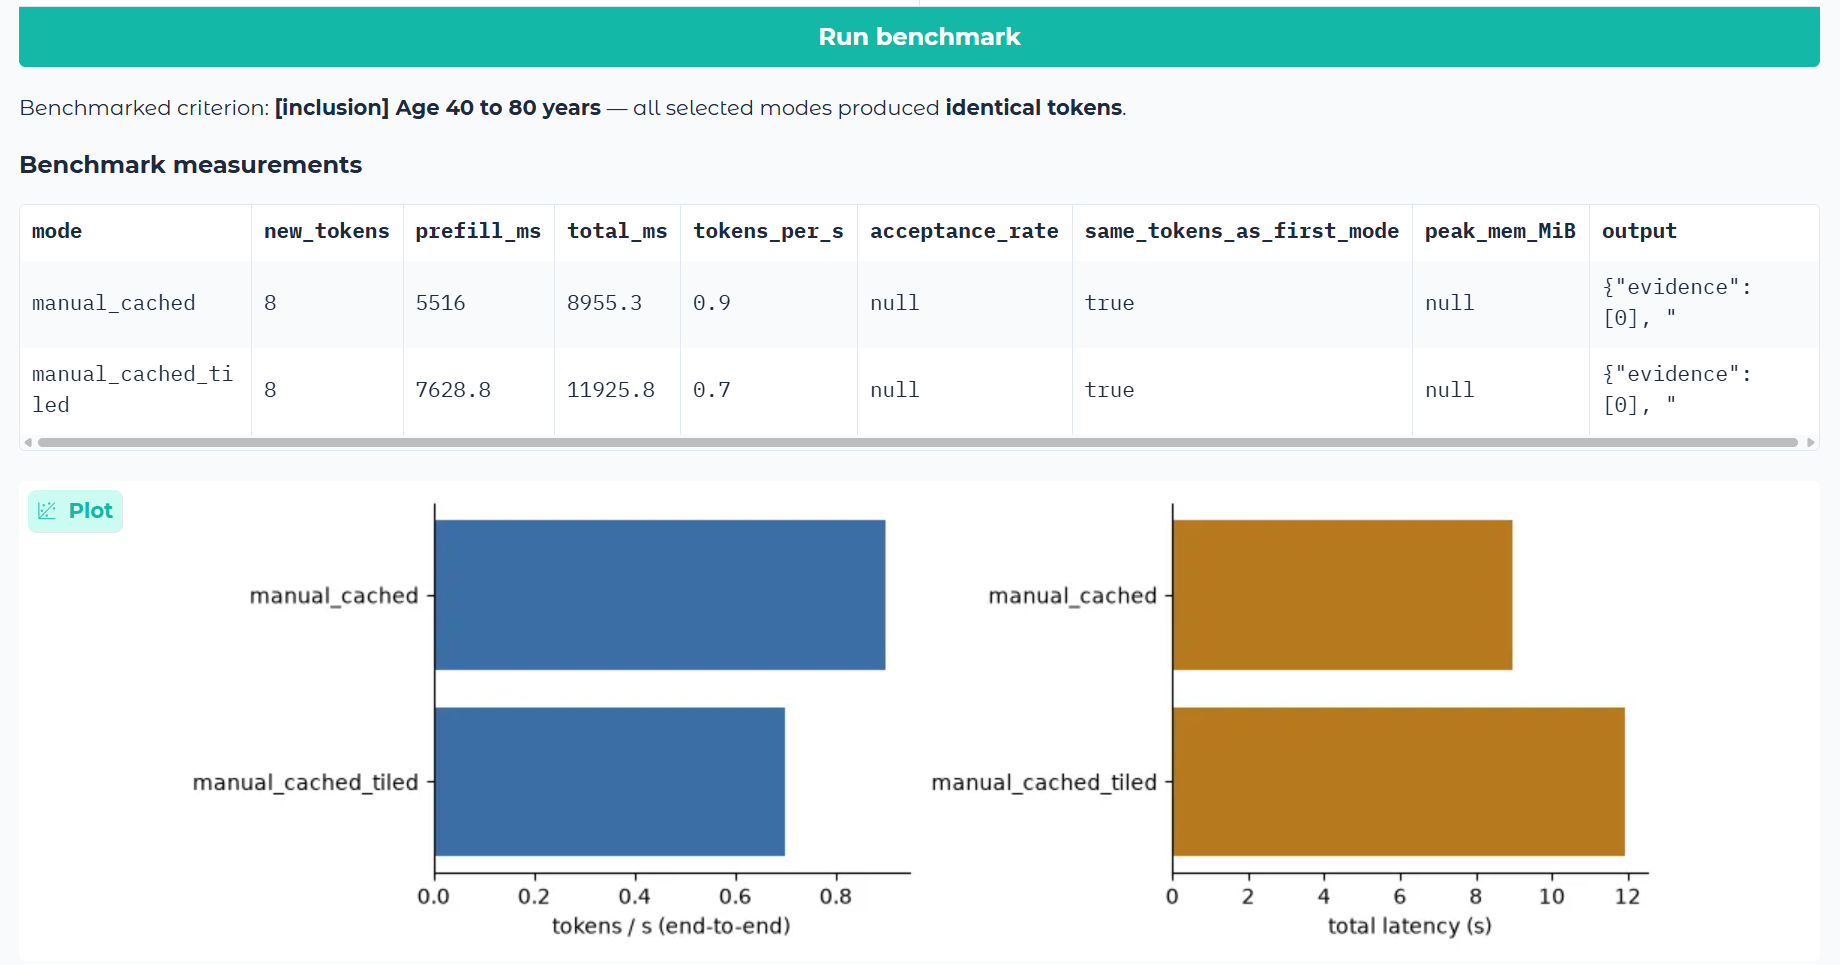
\includegraphics[width=\linewidth]{figures/app_benchmark.png}\\[-1pt]{\footnotesize (d) Live benchmark with token-equality check}
\end{minipage}
\caption{TrialMatch browser application (CPU laptop, FP32, fine-tuned adapters loaded). Exported HTML/JSON reports contain the same content plus provenance.}
\label{fig:app}
\end{figure*}

% ======================================================================
\section{Limitations}
\begin{itemize}
\item \textbf{Small test set.} Eight test patients (206 correlated annotations) give wide intervals (fine-tuned test accuracy 0.62--0.84); validation macro-F1 gains are not significant, and \emph{excluded} cannot be evaluated on test.
\item \textbf{Class collapse.} The model never predicts \emph{not included}, \emph{excluded} or \NA, and answers \emph{not excluded} for every exclusion criterion. Class-weighted loss or oversampling were not tried because the test set had already been used; they are the obvious next step and must be selected on validation.
\item \textbf{Absence treated as a negative.} The model has learned the annotation convention that an unmentioned exclusion is \emph{not excluded}, which conflicts with the screening principle that missing information is not proof.
\item \textbf{Reasoning depth.} Numeric thresholds and multi-step clinical inference (shock from vital signs, HbA1c ranges) remain unreliable at 1.5B parameters.
\item \textbf{Inference speed.} Our decoders are educational PyTorch code; tiled attention and speculative decoding are correct but slower than fused or greedy baselines on a T4, and BF16 timings are affected by emulation.
\item \textbf{Scope.} The aggregation rule is not validated against patient-level ground truth, which the dataset does not provide; the system is a research prototype, not a clinical decision tool.
\end{itemize}

% ======================================================================
\section{Conclusion}
TrialMatch shows that a 1.5B open-weight decoder, adapted with 18.5\,M LoRA parameters on a free GPU, can perform criterion-level eligibility screening with sentence-level evidence. On held-out patients it reaches 0.733 accuracy and 0.601 evidence micro-F1, against 0.267 and 0.136 before fine-tuning. A majority baseline and per-class analysis show that this gain is concentrated on inclusion criteria, while rare classes and exclusion decisions remain the main open problem. The inference work shows that each mechanism can be implemented from first principles and verified: an owned KV cache with exact FP32 agreement and a 32$\times$ decode speed-up, an online-softmax tiled kernel with 57$\times$ lower attention memory, and speculative decoding that provably preserves greedy output, with its slowdown on this hardware explained quantitatively. Future work should address class imbalance with validation-selected reweighting, use larger target-to-draft ratios for speculative decoding, and validate the aggregation rule against patient-level trial outcomes.

% ======================================================================
\begin{thebibliography}{99}
\bibitem{jin2024trialgpt} Q.~Jin, Z.~Wang, C.~S. Floudas, F.~Chen, C.~Gong, D.~Bracken-Clarke, E.~Xue, Y.~Yang, J.~Sun, and Z.~Lu, ``Matching patients to clinical trials with large language models,'' \emph{Nature Communications}, vol.~15, Art.~no.~9074, 2024.
\bibitem{koopman2016} B.~Koopman and G.~Zuccon, ``A test collection for matching patients to clinical trials,'' in \emph{Proc.\ 39th Int.\ ACM SIGIR Conf.\ Research and Development in Information Retrieval}, 2016, pp.~669--672.
\bibitem{wong2023scaling} C.~Wong, S.~Zhang, Y.~Gu, C.~Moung, J.~Abel, N.~Usuyama, R.~Weerasinghe, B.~Piening, T.~Naumann, C.~Bifulco, and H.~Poon, ``Scaling clinical trial matching using large language models: A case study in oncology,'' in \emph{Proc.\ Machine Learning for Healthcare Conf.}, PMLR vol.~219, 2023.
\bibitem{vaswani2017} A.~Vaswani, N.~Shazeer, N.~Parmar, J.~Uszkoreit, L.~Jones, A.~N. Gomez, {\L}.~Kaiser, and I.~Polosukhin, ``Attention is all you need,'' in \emph{Advances in Neural Information Processing Systems}, vol.~30, 2017.
\bibitem{qwen25} Qwen Team (A.~Yang \emph{et~al.}), ``Qwen2.5 technical report,'' arXiv:2412.15115, 2024.
\bibitem{llama3} A.~Grattafiori \emph{et~al.}, ``The Llama 3 herd of models,'' arXiv:2407.21783, 2024.
\bibitem{smollm2} L.~B. Allal \emph{et~al.}, ``SmolLM2: When smol goes big---Data-centric training of a small language model,'' arXiv:2502.02737, 2025.
\bibitem{su2024roformer} J.~Su, M.~Ahmed, Y.~Lu, S.~Pan, W.~Bo, and Y.~Liu, ``RoFormer: Enhanced transformer with rotary position embedding,'' \emph{Neurocomputing}, vol.~568, Art.~no.~127063, 2024.
\bibitem{ainslie2023gqa} J.~Ainslie, J.~Lee-Thorp, M.~de~Jong, Y.~Zemlyanskiy, F.~Lebr{\'o}n, and S.~Sanghai, ``GQA: Training generalized multi-query transformer models from multi-head checkpoints,'' in \emph{Proc.\ Conf.\ Empirical Methods in Natural Language Processing (EMNLP)}, 2023.
\bibitem{shazeer2019} N.~Shazeer, ``Fast transformer decoding: One write-head is all you need,'' arXiv:1911.02150, 2019.
\bibitem{hu2022lora} E.~J. Hu, Y.~Shen, P.~Wallis, Z.~Allen-Zhu, Y.~Li, S.~Wang, L.~Wang, and W.~Chen, ``LoRA: Low-rank adaptation of large language models,'' in \emph{Proc.\ Int.\ Conf.\ Learning Representations (ICLR)}, 2022.
\bibitem{dettmers2023qlora} T.~Dettmers, A.~Pagnoni, A.~Holtzman, and L.~Zettlemoyer, ``QLoRA: Efficient finetuning of quantized LLMs,'' in \emph{Advances in Neural Information Processing Systems}, vol.~36, 2023.
\bibitem{loshchilov2019adamw} I.~Loshchilov and F.~Hutter, ``Decoupled weight decay regularization,'' in \emph{Proc.\ Int.\ Conf.\ Learning Representations (ICLR)}, 2019.
\bibitem{pope2023} R.~Pope, S.~Douglas, A.~Chowdhery, J.~Devlin, J.~Bradbury, J.~Heek, K.~Xiao, S.~Agrawal, and J.~Dean, ``Efficiently scaling transformer inference,'' in \emph{Proc.\ Machine Learning and Systems (MLSys)}, vol.~5, 2023.
\bibitem{kwon2023paged} W.~Kwon, Z.~Li, S.~Zhuang, Y.~Sheng, L.~Zheng, C.~H. Yu, J.~E. Gonzalez, H.~Zhang, and I.~Stoica, ``Efficient memory management for large language model serving with PagedAttention,'' in \emph{Proc.\ 29th ACM Symp.\ Operating Systems Principles (SOSP)}, 2023.
\bibitem{milakov2018} M.~Milakov and N.~Gimelshein, ``Online normalizer calculation for softmax,'' arXiv:1805.02867, 2018.
\bibitem{rabe2021} M.~N. Rabe and C.~Staats, ``Self-attention does not need $O(n^2)$ memory,'' arXiv:2112.05682, 2021.
\bibitem{dao2022flash} T.~Dao, D.~Y. Fu, S.~Ermon, A.~Rudra, and C.~R{\'e}, ``FlashAttention: Fast and memory-efficient exact attention with IO-awareness,'' in \emph{Advances in Neural Information Processing Systems}, vol.~35, 2022.
\bibitem{dao2023flash2} T.~Dao, ``FlashAttention-2: Faster attention with better parallelism and work partitioning,'' in \emph{Proc.\ Int.\ Conf.\ Learning Representations (ICLR)}, 2024.
\bibitem{leviathan2023} Y.~Leviathan, M.~Kalman, and Y.~Matias, ``Fast inference from transformers via speculative decoding,'' in \emph{Proc.\ 40th Int.\ Conf.\ Machine Learning (ICML)}, PMLR vol.~202, 2023, pp.~19274--19286.
\bibitem{chen2023spec} C.~Chen, S.~Borgeaud, G.~Irving, J.-B. Lespiau, L.~Sifre, and J.~Jumper, ``Accelerating large language model decoding with speculative sampling,'' arXiv:2302.01318, 2023.
\bibitem{wolf2020transformers} T.~Wolf \emph{et~al.}, ``Transformers: State-of-the-art natural language processing,'' in \emph{Proc.\ Conf.\ Empirical Methods in Natural Language Processing: System Demonstrations}, 2020, pp.~38--45.
\end{thebibliography}

% ======================================================================
\appendices
\section{Reproducibility}
{\renewcommand\UrlFont{\footnotesize\ttfamily}
\begin{itemize}
\item \textbf{Source code and results:}\\ \url{https://github.com/eshaalmk/genai-a2-trialmatch}\\
Includes \texttt{requirements.txt}, data preparation, training, evaluation and benchmark scripts, the split manifest (\texttt{results/data/}), training logs and all benchmark results.
\item \textbf{Target adapter (Qwen2.5-1.5B + LoRA):}\\ \url{https://drive.google.com/drive/folders/1JRlnBXRM27rMjB_yDv0fb6_HaL7KxghY}
\item \textbf{Draft adapter (Qwen2.5-0.5B + LoRA):}\\ \url{https://drive.google.com/drive/folders/1PLednYrQxz02hfXREQLlTyw5Ws0dRuy8}
\item \textbf{Demonstration video:}\\ \url{https://drive.google.com/file/d/1AYAB7_aVrXotf8DfoxDOyJ67W0fcUtE8/view}
\item \textbf{Reproducing the experiments:} run the Colab notebook in \texttt{notebooks/} on a T4 GPU; checkpoints are saved to Google Drive and training resumes after a disconnect.
\item \textbf{Running the application:} place the adapters in \texttt{weights/} and double-click \texttt{start\_app.bat} (Windows) or run \texttt{start\_app.sh} (macOS/Linux); the app opens at \texttt{127.0.0.1:7860}.
\end{itemize}}

\section{AI-Use Statement}
Claude (Anthropic) was used as a coding and writing assistant: to scaffold the repository, the training and evaluation scripts, the manual decoder, the attention and speculative-decoding implementations, the application and the notebook, to review experimental results, and to help draft this report. All experiments were run by the author on Google Colab and a personal laptop; all numbers in this report are taken from the result files produced by those runs. The generated code was tested with unit tests, token-equality tests against Hugging Face reference decoding, and FP64 numerical tests. During review, problems were found and fixed, including the inherited repetition penalty, the BF16 device selection and the parameter-count error. The author is responsible for the submission and can explain and modify each component.

\end{document}
